\section{Prospettive sulla programmazione parallela}
Uno degli aspetti più importanti della programmazione parallela, è analizzare il problema e capire se può essere parallelizzato. La parallelizzazione del codice porta a dei miglioramenti delle performance solo se il workload (peso computazionale) è non trascurabile.
Seguono alcune definizioni
\begin{itemize}
    \item \textbf{Task: } unità di esecuzione o di lavoro di un programma o di un sottoprogramma. Le istruzioni sono eseguite sequenzialmente ovvero non in parallelo.

    \item Processo/thread: entità astratta che esegue i task assegnati ai processi. I processi comunicano tra di loro e si sincronizzano per eseguire i loro task.
    \item Processore: motore fisico su cui ciascun processo viene eseguito. Il programma viene scritto come un insieme di processi che vengono poi mappati sul processore.
\end{itemize}

\subsection{Step per creare un programma parallelo}
\begin{figure}[th]
	\centering
	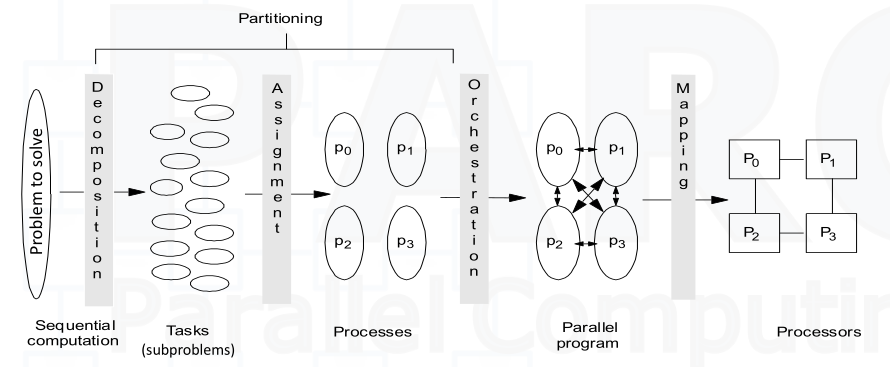
\includegraphics[width=0.7\linewidth]{img/4-step-programma-parallelo}
	\caption{i 4 step per creare un programma parallelo.}
	\label{fig:4-step-programma-parallelo}
\end{figure}

Ci sono 4 passi nella creazione di un programma parallelo:
\begin{enumerate}
    \item Decomposizione dell'algoritmo risolutivo in task o sottoproblemi;
    \item Si assegnano le varie task ai processi; 
    \item Orchestrazione dell'accesso ai dati, comunicazione e sincronizzazione  da parte dei processi;
    \item Mapping dei processi ai processori ()un processo non può essere assegnato a più unità di calcolo).
\end{enumerate}

Il livello di parallelismo viene determinato nelle fasi di decomposizione e assegnamento.

\subsubsection{Comprensione del problema/programma}
Indubbiamente, il primo passo nello sviluppo di software parallelo è capire innanzitutto il problema che si desidera risolvere in parallelo. Se si parte da un programma seriale, ciò implica anche la comprensione del codice esistente.

Prima di investire tempo nel tentativo di sviluppare una soluzione parallela per un problema, bisogna determinare se il problema può effettivamente essere parallelizzato.


\begin{enumerate}
    \item Identificare gli \textbf{hotspot} del programma: rappresentano le parti dove viene svolta la maggior parte del lavoro effettivo. La maggior parte dei programmi scientifici e tecnici di solito svolgono la maggior parte del loro lavoro in pochi punti. Gli strumenti di profilazione e analisi delle prestazioni possono aiutare ad individuare gli hotspote .profiling\footnote{I tool di profiling eseguono il codice e, assieme al suo risultato, ritornano anche un report che può contenere: il numero di invocazioni per ogni funzione contenuta nel codice, e il tempo che impiega ciascuna per determinare il risultato che calcola, quali sono le parti del codice più usate, e così via,\dots} e analisi delle performance (tramite appositi tool). Gli hotspot sono generalmente le sezioni in cui si concentra la parallelizzazione e che hanno un utilizzo della CPU alto.
    \item Identificare i \textbf{bottleneck} del programma: sono le aree di codice che sono più lente da eseguire (come ad esempio le sezioni dedicate all'I/O). Una possibile strada che si può seguire per contrastare i bottleneck, consiste nel trasferire la loro esecuzione sulla GPU, in modo da non dover rallentare la CPU. Dunque, si possono vedere due livelli di parallelismo: il primo dato dalla parallelizzazione su GPU del codice, mentre il secondo dato dalla concorrenza di esecuzione di CPU e GPU.
    \item Identificare gli\textbf{ inibitori al parallelismo}: analizzare il problema significa anche identificare gli inibitori del parallelismo, che sono quei fattori che impediscono di parallelizzare il codice. Una classe comune di inibitori è la dipendenza dei dati, come dimostrato dalla sequenza di Fibonacci sotto.
\end{enumerate}

\underline{Esempio di problema parallelizzabile}: Calcolare l'energia potenziale per migliaia di diverse conformazioni molecolari indipendenti. Una volta completato, individua la conformazione molecolare con l'energia potenziale minima. Ogni conformazione molecolare è determinabile in modo indipendente e il calcolo dell'energia potenziale minima è parallelizzabile.
\\

\underline{Esempio di problema non-parallelizzabile}: Calcolare la serie di Fibonacci. Questo problema non è parallelizzabile in quanto il calcolo attuale dipende dai calcoli precedenti (il termine $k+2$ è dato dalla somma dei termini $k+1$ e $k$). 
\\



\subsubsection{Decomposizione}
Nella decomposizione (o scomposizione) di un problema in task, è cruciale individuarne un numero appropriato in modo che ci siano sempre thread sufficienti per mantenere i processori occupati. In una configurazione con 100 processori funzionanti in parallelo, è necessario avere un ampio pool di task per garantire che tutti i processori siano costantemente utilizzati, anche se uno dei compiti si blocca. È comune che un task raggiunga un punto in cui necessita di dati da un altro task o deve eseguire operazioni di I/O, interrompendo temporaneamente l'esecuzione e lasciando il processore inutilizzato. L'obiettivo è minimizzare questa inattività, assicurando che un nuovo task sia pronto per essere eseguito non appena un processore si libera. Ogni core o processore lasciato inattivo rappresenta uno spreco di risorse. Pertanto, è essenziale disporre di un numero sufficiente di task prontamente disponibili per sostituire quelli bloccati e massimizzare l'utilizzo dei processori.

Esistono due modi per scomporre in task:
\begin{itemize}
    \item Scomposizione di dominio: prevede di scomporre i dati del problema, facendo lavorare poi ogni task su una porzione dei dati. Esistono vari modi di partizionare i dati, la soluzione migliore generalmente dipende dal modo in cui sono memorizzati i dati.

    I problemi, che siano monodimensionale che bidimensionali, possono essere scomposti, ad esempio, in blocchi o cicli (figure \ref{fig:domain-decomposition}). Un fattore importante da tenere presente è il bilanciamento del carico (\textbf{load balancing}). se siamo sicuri che il tempo impiegato dalla prima thread sul blocco A corrisponde a quello impiegato dalla seconda thread sul blocco B e così via per il resto dei blocchi, allora abbiamo un carico bilanciato. Questo di solito è il caso per problemi lineari. Quando però abbiamo problemi più complessi, il carico di lavoro di una thread diventa imprevedibile. In questo caso potrebbe essere più ottimale aumentare i blocchi facendo in modo che il primo processore che si libera vada a prendere la successiva thread in attesa.
    \begin{figure}[th]
    	\centering
    	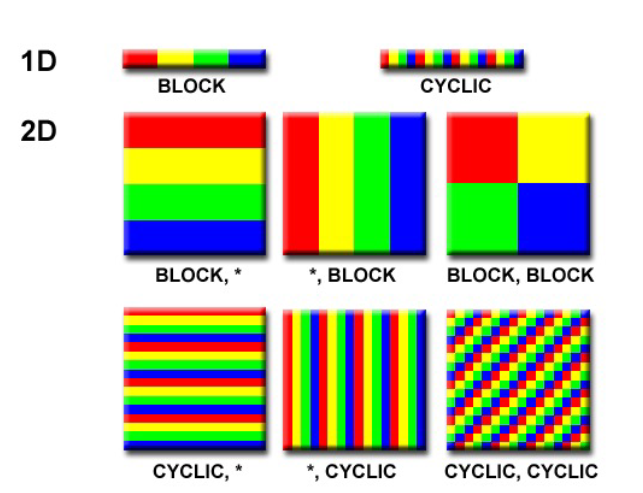
\includegraphics[width=0.7\linewidth]{img/domain-decomposition.png}
    	\caption{Esempio di decomposizione del dominio.}
    	\label{fig:domain-decomposition}
    \end{figure}

    \item Scomposizione funzionale: ci si concentra sull'elaborazione che deve essere fatta piuttosto che sui dati manipolati dalla computazione. Il problema è quindi scomposto rispetto al lavoro che deve essere fatto. Ogni task esegue parte del lavoro totale.
\end{itemize}

La scomposizione è compito del programmatore, che può essere supportato da tool automatici (campo di ricerca).

\underline{Esempio di parallelizzazione}
\\

Data un'immagine $N\times N$ vogliamo:
\begin{enumerate}[label=$\bullet$ \textbf{Step \arabic*:}]
    \item raddoppiare la luminosità di ogni pixel; {\color{NavyBlue}\textbf{(complessità $N^2$)}}
    \item calcolare la media di tutti i pixel. {\color{NavyBlue}\textbf{(complessità $N^2$)}}
\end{enumerate}

\paragraph{Soluzione sequenziale.} Una soluzione sequenziale di questo problema costa un tempo totale di {\color{NavyBlue}$N^2+N^2=2N^2$} (figura \ref{fig:esecuzione-sequenziale}). 
\begin{figure}[th]
	\centering
	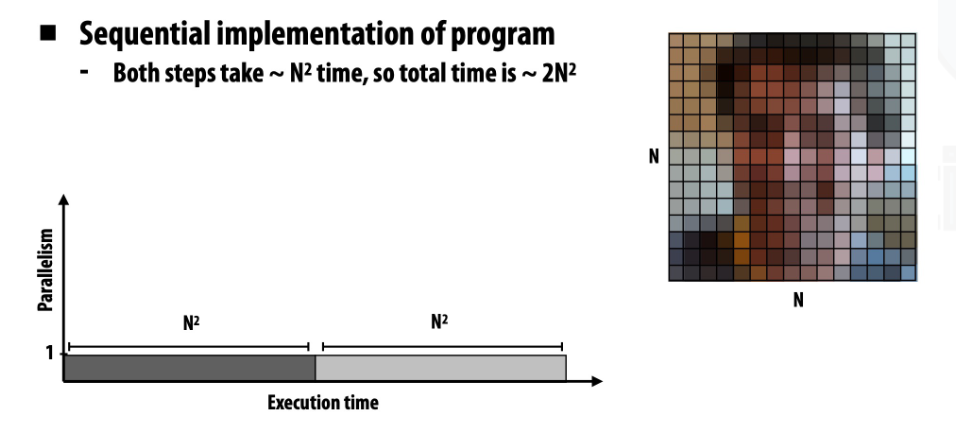
\includegraphics[width=0.7\linewidth]{img/esecuzione-sequenziale.png}
	\caption{Esecuzione sequenziale.}
	\label{fig:esecuzione-sequenziale}
\end{figure}

\paragraph{Parallelizzazione sulla prima fase.}Una strategia di parallelizzazione consiste nell'eseguire in parallelo lo step 1, completandolo in $\frac{N^2}{P}$ (figure \ref{fig:esecuzione-parallela-1}), dove $P$ rappresenta il numero di processori disponibili. Invece parallelizzare lo step 2 risulta inefficiente  per via della interdipendenza tra i pixel dell'immagine nell'applicazione del filtro, dunque il suo costo è di $N^2$. Lo speedup stimato risulta:
\begin{align*}
    speedup &\le \frac{2N^2}{\frac{N^2}{P} + N^2}\\
    &\le 2
\end{align*}

\begin{figure}[th]
	\centering
	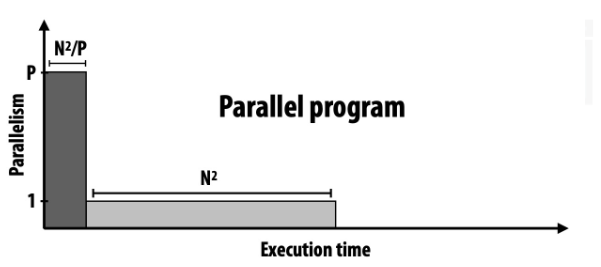
\includegraphics[width=0.7\linewidth]{img/esecuzione-parallela-1.png}
	\caption{Primo tentativo di parallelismo.}
	\label{fig:esecuzione-parallela-1}
\end{figure}

\paragraph{Parallelizzazione sulla seconda fase}Un miglioramento potrebbe essere ottenuto parallelizzando il calcolo della media su ${P}$ processori (calcolo su $P$ matrici di dimensione $\frac{ N^2}{P}$ -- figura \ref{fig:esecuzione-parallela-2}). Infine viene introdotto un tempo di overhead dovuto alla combinazione delle somme parallele per ottenere il risultato finale. I tempi diventano:
\begin{align*}
    \text{Tempo step 1 } &= \frac{N^2}{P}\\
    \text{Tempo step 2 } &= \frac{N^2}{P}+P    
\end{align*}

e si ottiene uno speedup pari a:
\begin{align*}
    speedup \le \frac{2N^2}{\frac{2N^2}{P} + P}\\
\end{align*}

\begin{figure}[th]
	\centering
	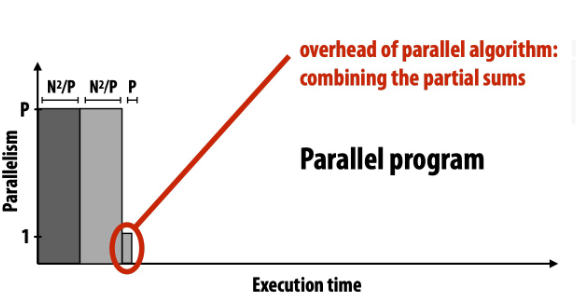
\includegraphics[width=0.7\linewidth]{img/esecuzione-parallela-2.png}
	\caption{Secondo tentativo di parallelismo.}
	\label{fig:esecuzione-parallela-2}
\end{figure}

\subsubsection{Assegnamento}
In questa fase andiamo a specificare il meccanismo con cui dividere le task tra i processi. Per semplicità, possiamo vedere le task come "cose da fare", mentre i processi/thread come i "lavoratori". Abbiamo fatto la scomposizione, sappiamo quanti e quali sono le thread, cerchiamo ora di fare un assegnamento che ci garantisca un certo livello di carico. 
Un approccio strutturato solitamente funziona bene, possiamo seguire euristiche ben conosciute o anche ispezionare attentamente il codice.


Il \textbf{load balancing} (bilanciamento del carico di lavoro) fa riferimento alla pratica di distribuzione delle task tra le thread affinchè tutte le thread siano occupate tutto il tempo. Possiamo anche definirlo come la riduzione al minimo dei tempi di inattività del processo. Questo passo è molto significativo per le perfromance. Ad esempio, se tutti i processi fossero soggetti ad un punto che funge da barriera di sincronizzazione, le performance globali verrebbero determinate dalla task più lenta.
\begin{figure}[th]
	\centering
	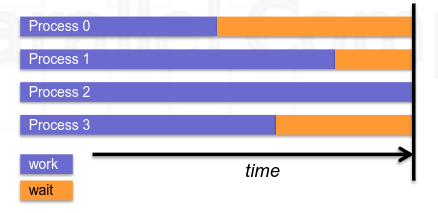
\includegraphics[width=0.7\linewidth]{img/barrier-sync.png}
	\caption{Esempi di punto di sincronizzazione.}
	\label{fig:barrier-sync}
\end{figure}

Possiamo ottenere il load balancing in più modi:
\begin{enumerate}
    \item Dividendo equamente le task tra i processi disponibili:
    \begin{itemize}
        \item In caso di operazioni su array/matrici, dove ogni processo esegue operazioni simili, il dataset viene distribuito in modo uniforme tra i processi;
        \item Per le iterazioni di un ciclo dove il lavoro svolto da ogni loop è similare, le iterazioni vengono distribuite uniformemente tra i processi;
        \item Se si utilizza un mix eterogeneo di macchine con performance variabili, è consigliato utilizzare dei tool di analisi delle performance per individuare carichi sbilanciati e aggiustare di conseguenza.
    \end{itemize}
    \item Usando un assegnamento dinamico del lavoro: alcune classi generano un carico di lavoro sbilanciato anche se i dati sono distribuiti egualmente tra il processi, come:
    \begin{itemize}
        \item Array sparsi;
        \item Adaptive grid methods, dove alcuni processi potrebbero dover perfezionare la propria mesh, mentre altri no;
        \item N-body simulations, dove alcune particelle potrebbero migrare verso/dal dominio del proprio processo di origine verso quello di un altro processo, oppure dove alcune particelle richiedono più lavoro rispetto ad altre.
    \end{itemize}
    Quando l'ammontare di lavoro che ogni thread performerà è variabile (non intenzionalmente ovviamente), è utile usare un approccio \textbf{scheduler – task pool}. In questo modo, appena un processo finisce, si mette in coda per ottenere un nuovo pezzo di lavoro.
    Inoltre, potrebbe diventare necessario disegnare un algoritmo che rileva e gestire sbilanciamento mentre questi si verificano dinamicamente nel codice.
\end{enumerate}

La \textbf{granularità} rappresenta una misura qualitativa del rapporto tra computazione e comunicazione. Generalmente i periodi di computazione sono separati da quelli di comunicazione da eventi di sincronizzazione. Relativamente al parallelismo, la granularità si divide in:
\begin{itemize}
    \item Fine grain parallelism (parallelismo a grana fine): si effettuano relativamente piccole quantità di lavoro computazionale tra gli eventi di comunicazione. Abbiamo quindi un basso rateo tra computazione e comunicazione. Facilita il load balancing; implica un elevato overhead di comunicazione e meno opportunità per il miglioramento delle performance. Se la granularità è troppo fine è possibile che l'overhead richiesto per comunicazione ee sincronizzazione tra le task richieda più tempo della computazione vera e propria.





    \item Coarse grain parallelism (parallelismo a grana grossa): si effettuano relativamente grandi quantità di lavoro computazionale tra gli eventi di comunicazione/sincronizzazione. Abbiamo quindi un alto rateo tra computazione e comunicazione. Implica più opportunità per un incremento delle performance, ma rende più difficile bilanciare il carico di lavoro efficientemente
\end{itemize}










